% This is LLNCS.DEM the demonstration file of
% the LaTeX macro package from Springer-Verlag
% for Lecture Notes in Computer Science,
% version 2.4 for LaTeX2e as of 16. April 2010
%
\documentclass{llncs}
%
\usepackage{amsmath}
\usepackage{amssymb}
\usepackage{tikz}
\usepackage[linesnumbered,ruled]{algorithm2e}
\usepackage{graphicx}
\usepackage{subfig}

\newcounter{instr}
\newcommand{\ninstr}{\refstepcounter{instr}\theinstr.}

\begin{document}

\title{Kassian score}

\titlerunning{Kassian score}

%\author{Tom\'{a}\v{s} Flouri\inst{1} \and Paschalia Kapli\inst{1} \and Sarah Lutteropp\inst{1}}
\authorrunning{Tom\'{a}\v{s} Flouri et al.} % abbreviated author list
\institute{Heidelberg Institute of Theoretical Studies}

\maketitle

\begin{abstract}
An explanation of the Kassian score.
\end{abstract}

\section{Kassian Score}
In order to compare the maximum likelihood delimitation model with the known real species assignments, we defined the \emph{Kassian Score}. Given two sets of most recent common ancestors (MRCAs) and a phylogenetic tree, the Kassian Score counts the minimum number of movements in the tree needed to transform the one set of MRCAs into the other. We considered two possible moves. The first move is that a MRCA node can be pushed one layer downwards, turning its children nodes into MRCAs instead. The second move is that a MRCA node can be pulled one layer downwards, turning its parent node into a MRCA instead. Figure~\ref{fig:movements} shows both possible moves.

\begin{figure}[H!]
\centering
\subfloat[Before moving the node $b$ upwards in the tree, the nodes $b$ and $c$ are MRCAs. After the upward move, $a$ is the only MRCA in the subtree.]{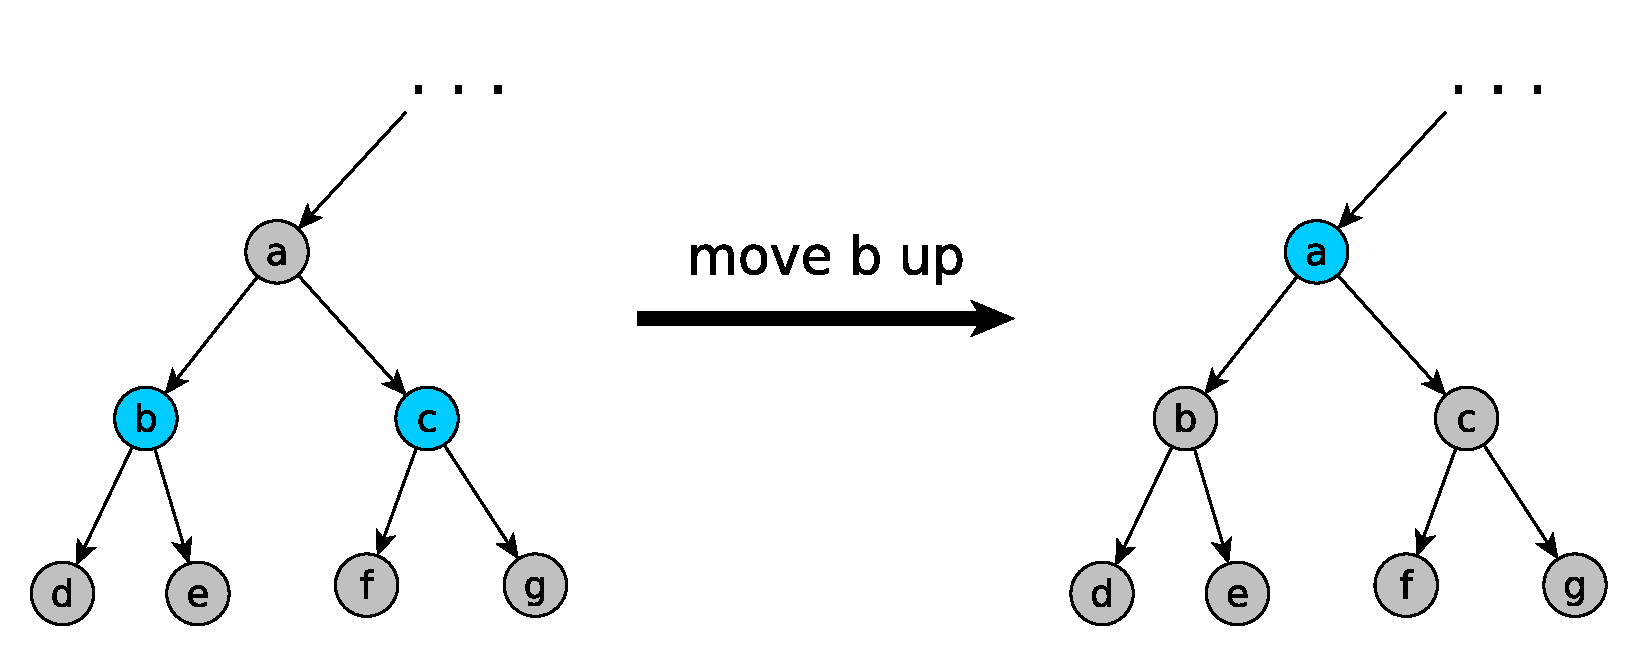
\includegraphics[scale=0.35]{images/move_up.pdf}} 

\subfloat[Before pushing the node $b$ down in the tree, the nodes $b$ and $c$ are MRCAs. After the downward move, $d$, $e$ and $c$ are the MRCAs in the subtree.]{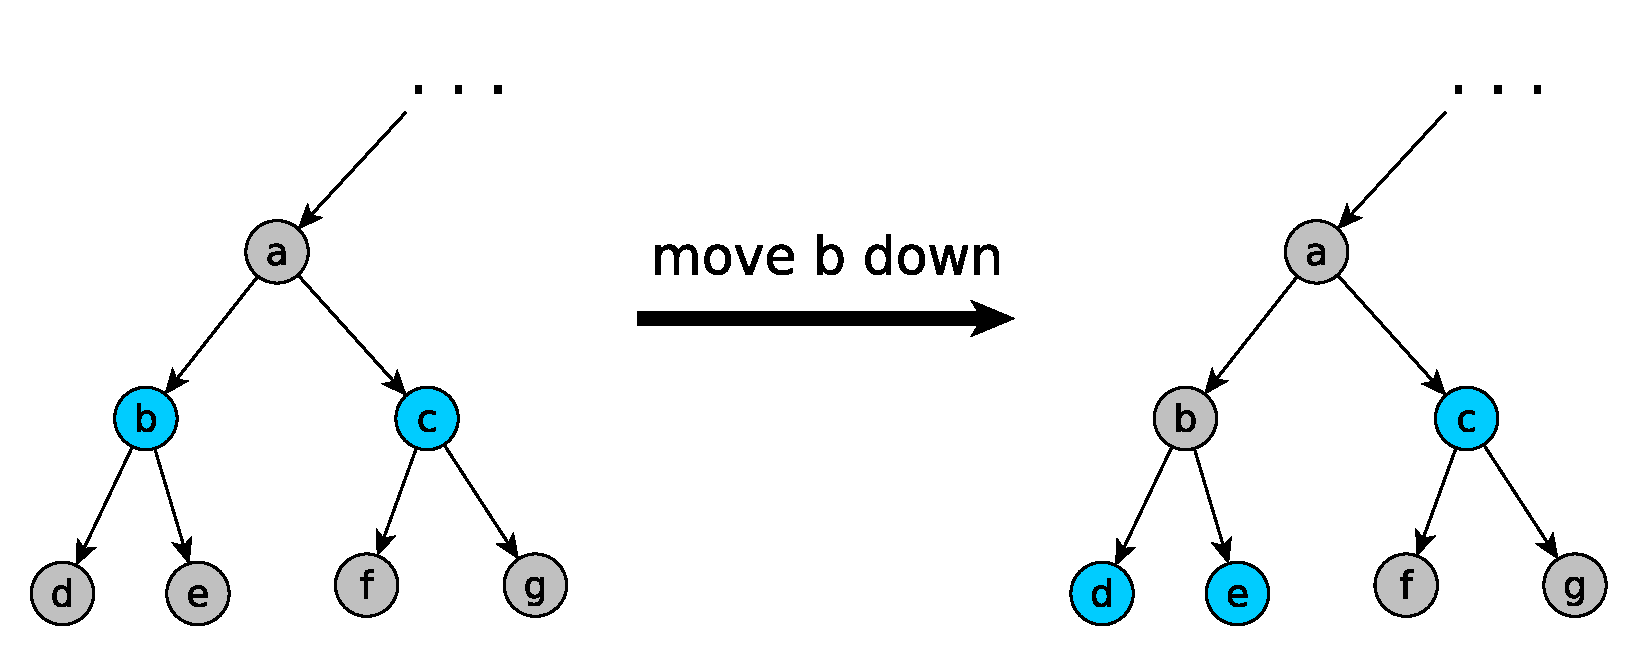
\includegraphics[scale=0.35]{images/move_down.pdf}} 
   
\caption{The possible moves in the Kassian Score. In each movement step, a MRCA node can either be moved one layer up or one layer down in the tree.}
\label{fig:movements}
\end{figure}

\paragraph{Computation}
In order to compute the Kassian Score, we used the following trick. In a first step, we marked all MRCA nodes from either the first set or the second set of MRCAs in the tree. Starting from each marked node, we followed the path from it to the root of the tree, counting the number of edges taken. If we encountered another marked node on our way, the number of edges already taken was added as a penalty to the Kassian Score. Algorithm~\ref{algo:kassianscore} shows the pseudocode of this approach.

\begin{algorithm}
\SetKwInOut{Input}{Input}
\SetKwInOut{Output}{Output}

\Input{A phylogenetic tree $T$ with edges $E$ and nodes $V$, a node $v$}
\Output{The number of edges taken until a MRCA node other than $v$ was visited on the path from $v$ to the root of $T$}

\underline{function findPenalty $(T, v)$}\\
penalty $\gets$ $0$\;

steps $\gets$ $0$\;
currentNode $\gets$ $v$\;
\While{currentNode $\neq$ root($T$)}{
  currentNode $\gets$ currentNode.parent\;
  steps $\gets$ steps + $1$\;
  \If{marked(currentNode)}{
     penalty $\gets$ steps\;
     \textbf{break}\;
  }
}
\Return{penalty}\;

\Input{A phylogenetic tree $T$ with edges $E$ and nodes $V$, a set of MRCA nodes $S_1$, a set of MRCA nodes $S_2$}
\Output{The minimum number of moves needed to transform the given sets of MRCA nodes into each other}

\underline{function computeKassianScore $(T, S_1, S_2)$}\\

kassianScore $\gets$ $0$\;

\For{$v \in V$}{
    marked($v$) $\gets$ \textbf{false}\;
	\If{$v \in S_1$ \textbf{ or } $v \in S_2$}{
		marked($v$) $\gets$ \textbf{true}\;
	}
	\Else{
	    marked($v$) $\gets$ \textbf{false}\;
	}
}

\For{$v \in V$}{
    \If{marked($v$)}{
        kassianScore $\gets$ kassianScore + \textit{findPenalty}($v$)\;
    }
}

\Return{kassianScore}

\caption{Computation of the Kassian Score}
\label{algo:kassianscore}
\end{algorithm}

\section{Problem: The Computation is wrong!}
The pseudocode given in Algorithm~\ref{algo:kassianscore} returns a penalty that is too high. Consider the example in Figure~\ref{fig:problem}.

\begin{figure}[H!]
\centering
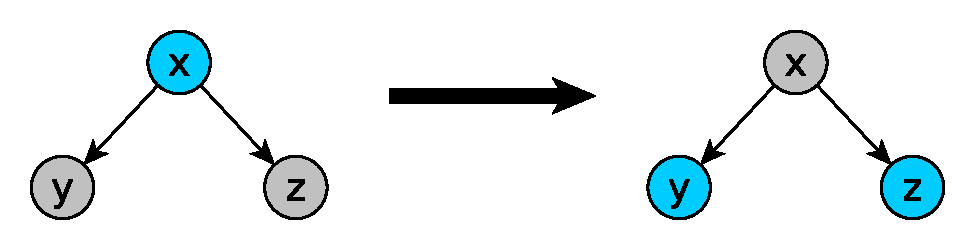
\includegraphics[scale=0.5]{images/problem_with_kassian_score.pdf}
\caption{Assume that we want to transform the MRCA set $S_1 = \{x\}$ into the MRCA set $S_2 = \{y,z\}$. We can do this by moving $x$ downwards, thus having to do only a single movement. The computation from Algorithm~\ref{algo:kassianscore} would return a Kassian Scor of $2$ moves, however.}
\label{fig:problem}
\end{figure}

\bibliographystyle{splncs03}
\bibliography{delimit}
\end{document}
